\documentclass[a4paper,11pt]{article}

\usepackage[utf8]{inputenc}

\usepackage{graphicx}
\usepackage{caption}
\usepackage{subcaption}

\usepackage{pgfplots}
\pgfplotsset{compat=1.18} 

\usepackage{minted}
\usepackage{siunitx}

\begin{document}

\title{
    \textbf{Performance of Array Operations in C}
}
\author{Mo Wang}
\date{Spring 2026}

\maketitle

\section*{Introduction}
This report investigates the performance of three fundamental array operations in C: random access of an element, linear search for a given key, and detection of duplicate elements in an array. The primary objective is to analyze how the execution time of these operations scales with the size of the array.

As part of an introduction to algorithms and data structures, this study emphasizes the practical aspects of algorithmic behavior by measuring elapsed time for each operation under varying input sizes. The results will be compared to theoretical expectations: constant time for random access ($O(1)$), linear time for search ($O(n)$), and quadratic time for duplicate detection ($O(n^2)$).

\section*{Benchmarking Methodology}

To measure execution time, the POSIX monotonic clock (\texttt{CLOCK\_MONOTONIC}) is used. This clock provides a high-resolution, non-adjustable time source suitable for benchmarking. Timing is performed by calling \texttt{clock\_gettime()} before and after the operation under test, storing the timestamps in \texttt{t\_start} and \texttt{t\_end} of type \texttt{struct timespec}.

The helper function \texttt{nano\_seconds()} computes the elapsed time in nanoseconds by taking pointers to \texttt{t\_start} and \texttt{t\_end} and returning the difference as a \texttt{long} integer:

\begin{minted}[breaklines]{C}
    long nano_seconds(struct timespec *t_start, struct timespec *t_stop) {
        return (t_stop->tv_nsec - t_start->tv_nsec) +
               (t_stop->tv_sec - t_start->tv_sec) * 1000000000;
    }

    // In one of three array benchmark functions:
    // code of allocating the memory for the array
    clock_gettime(CLOCK_MONOTONIC, &t_start);
    // code of one of three fundamental array operations
    clock_gettime(CLOCK_MONOTONIC, &t_stop);
    // code of cleaning up memory
    return nano_seconds(&t_start, &t_stop);
\end{minted}

However, the precision of \texttt{CLOCK\_MONOTONIC} is limited, typically on the order of hundreds of nanoseconds. This makes timing individual operations unreliable, especially for array access, which often completes in just a few nanoseconds. To mitigate this, each algorithm is executed repeatedly in a batch (in this case, 1024 iterations), and the total time is measured. The amortized time per operation is then estimated by dividing the total elapsed time by the number of iterations.

Execution time can also fluctuate due to hardware constraints, operating system scheduling, and background processes. To reduce noise, each benchmark is repeated multiple times (16 trials in this case), and the minimum elapsed time is reported as the most stable measure.

To prevent compiler optimizations from removing benchmark code as dead code, results are accumulated into a variable and accessed after the loop. Arrays are allocated on the heap and initialized with pseudo-random values to avoid cache locality and other optimizations that could distort measurements. For each benchmark, the array size doubles between tests to reveal scaling behavior and growth trends.

Finally, reported numbers use an appropriate number of significant digits (2 significant digits in this case). The goal is not to claim unrealistic precision but to illustrate clear performance trends as input size increases.

\section*{Random access}

In order to measure the elapsed time of random array access, an index array \texttt{index\_array} is first constructed and filled with pseudo-random indices. During the benchmark, each element of \texttt{index\_array} is used to access the corresponding element of the array \texttt{array}, measuring the time required for random access operations while excluding the random number generation delay.

In Table 1, where the benchmark results are shown, the random index access time remains constant at 2.3 to 2.4 ns with minimal fluctuations. However, a noticeable increase to 4.8~ns per operation is observed for an array size of 131072 elements, mostly because the array cannot fit inside L1 and L2 cache, resulting in additional memory latency.

\begin{table}[h]
\begin{center}
\begin{tabular}{l|c}
\textbf{Size of array} & \textbf{Time per operation (amortized)}\\
\hline
  1024   &  2.3 ns \\
  2048   &  2.4 ns \\
  4096   &  2.4 ns \\
  8192   &  2.3 ns \\
  16384  &  2.4 ns \\
  32768  &  2.3 ns \\
  65536  &  2.4 ns \\
  131072 &  4.8 ns \\
\end{tabular}
\caption{Constant time in random array access}
\label{tab:table1}
\end{center}
\end{table}

The constant-time behavior is illustrated in Figure 1, where a constant function $ y=2.4 $ provides the best fit for the measured data using least-squares regression. This concludes that the random array access operation has the time complexity of $ O(1) $, due to its constant-time behavior.

\begin{figure}
  \centering
  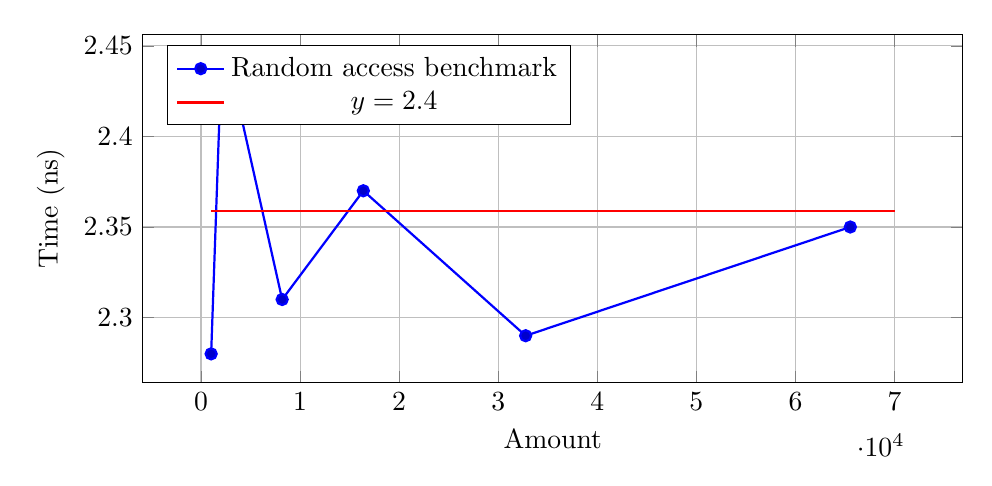
\begin{tikzpicture}
    \begin{axis}[
      xlabel={Amount},
      ylabel={Time (\si{\nano\second})},
      width=12cm, height=6cm,
      grid=major,
      legend pos=north west
    ]
      % Your benchmark data
      \addplot+[
        mark=*,
        thick,
        color=blue
      ] coordinates {
        (1024,   2.28)
        (2048,   2.44)
        (4096,   2.41)
        (8192,   2.31)
        (16384,  2.37)
        (32768,  2.29)
        (65536,  2.35)
      };
      \addlegendentry{Random access benchmark}

      \addplot[red, thick, domain=1000:70000] {2.359};
      \addlegendentry{$y = 2.4$}
      
    \end{axis}
  \end{tikzpicture}
  \caption{Random access benchmark with fitted line(s), x in array element size and y in time in nanoseconds}
  \label{fig:random-access}
\end{figure}

\section*{Linear search}

Benchmarking array search is similar to benchmarking random array access, but the randomly generated keys are compared sequentially against each element of the array until a match is found or the end of the array is reached.

In Table 2, judging the benchmark results, doubling the array size approximately doubles the execution time.

\begin{table}[h]
\begin{center}
\begin{tabular}{l|c}
\textbf{Size of array} & \textbf{Time per operation (amortized)}\\
\hline
  1024   &   1.7 µs   \\
  2048   &   3.3 µs   \\
  4096   &   6.4 µs   \\
  8192   &   13 µs    \\
  16384  &   26 µs    \\
  32768  &   51 µs    \\
  65536  &   100 µs   \\
  131072 &   200 µs   \\
\end{tabular}
\caption{Growing time in array search}
\label{tab:table1}
\end{center}
\end{table}

The fitted linear function in Figure 2 using least-squares regression in Figure 2 closely matches the measured data, with a small constant offset caused by loop overhead and control flow. This concludes that the time complexity of a linear array search is $ O(n) $, as the elapsed time grows linearly with the array size.

\begin{figure}
  \centering
  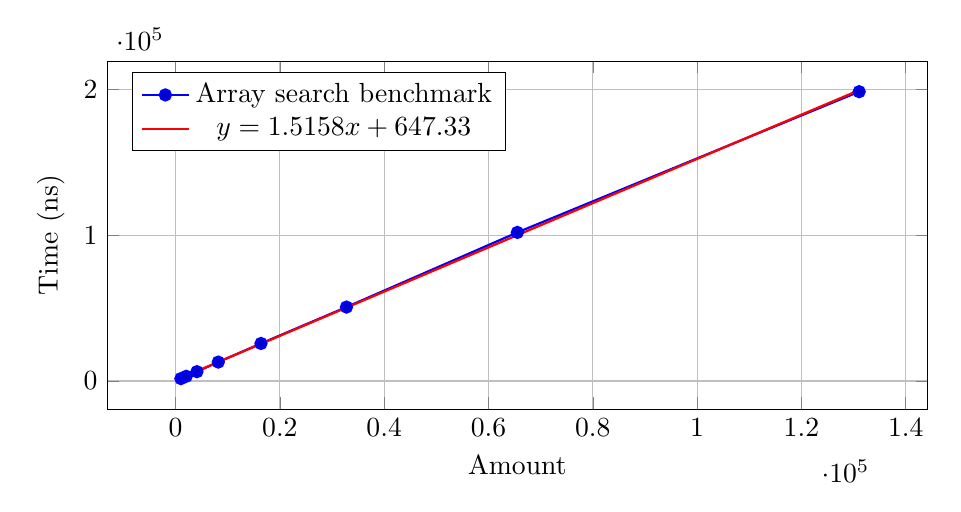
\begin{tikzpicture}
    \begin{axis}[
      xlabel={Amount},
      ylabel={Time (\si{\nano\second})},
      width=12cm, height=6cm,
      grid=major,
      legend pos=north west
    ]
      % Your benchmark data
      \addplot+[
        mark=*,
        thick,
        color=blue
      ] coordinates {
        (1024,   1679.10)
        (2048,   3268.07)
        (4096,   6436.80)
        (8192,   13010.31)
        (16384,  25751.70)
        (32768,  50693.34)
        (65536,  101850.42)
        (131072, 198295.30)
      };
      \addlegendentry{Array search benchmark}

      \addplot[red, thick, domain=0:131072] {1.5158*x + 647.33};
      \addlegendentry{$y = 1.5158x + 647.33$}
      
    \end{axis}
  \end{tikzpicture}
  \caption{Random access benchmark with fitted line(s)}
  \label{fig:random-access}
\end{figure}

\section*{Duplicate detection}

Measuring the duplication algorithm, an array is first allocated on the heap, filled with random numbers.
The algorithm takes the array and checks for duplicates by iterating through each element in the array and comparing it with all subsequent elements. The algorithm begins with the first element in the array. If a duplicate is found, the inner loop is exited early. Otherwise, the next element becomes the comparing element and the process continues.

In Table 3, the amortized time for each operation is roughly four times as large as the amount of elements in array doubles, by judging the benchmark result in time.

\begin{table}[h]
\begin{center}
\begin{tabular}{l|c}
\textbf{Size of array} & \textbf{Time (approximate)}\\
\hline
  1024   &  1.1 ms  \\  
  2048   &  3.7 ms  \\  
  4096   &  14 ms   \\ 
  8192   &  57 ms   \\ 
  16384  &  220 ms  \\  
  32768  &  890 ms  \\  
  65536  &  3.6 s   \\ 
  131072 &  14 s    \\
\end{tabular}
\caption{Quadratic time in array duplication checking algorithm}
\label{tab:table1}
\end{center}
\end{table}

Using least square-regression in figure 3, a quadratic time function produces a best fit to the given time measurements, with small linear and constant terms included in the model due to each loop overhead. As the array size increases, the term $ x^2 $ dominates in the fitted function, resulting into a $ O(n^2) $ time complexity.

\begin{figure}
  \centering
  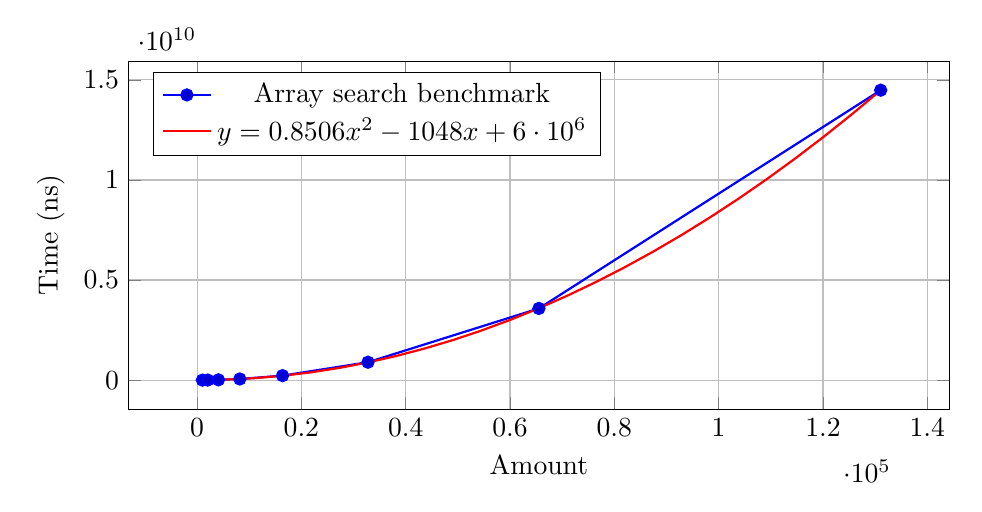
\begin{tikzpicture}
    \begin{axis}[
      xlabel={Amount},
      ylabel={Time (\si{\nano\second})},
      width=12cm, height=6cm,
      grid=major,
      legend pos=north west
    ]
      % Your benchmark data
      \addplot+[
        mark=*,
        thick,
        color=blue
      ] coordinates {
        (1024,   1065420.8)
        (2048,   3684608)
        (4096,   14206248.96)
        (8192,   56628264.96)
        (16384,  224418447.36)
        (32768,  894779381.76)
        (65536,  3580590469.12)
        (131072, 14484434739.2)
      };
      \addlegendentry{Array search benchmark}

      \addplot[red, thick, domain=0:131072] {0.8506*x^2 - 1048*x + 6e6};
      \addlegendentry{$y = 0.8506x^2 - 1048x + 6 \cdot 10^6$}
      
    \end{axis}
  \end{tikzpicture}
  \caption{Random access benchmark with fitted line(s)}
  \label{fig:random-access}
\end{figure}

\end{document}
